%%%%%%%%%%%%%%%%%%%%%%%%%%%%%%%%%%%%%%%%%%%%%%%%%%%%%%%%%%%
%%%%%%%%%%%%%%%%%%%%%%%%%%%%%%%%%%%%%%%%%%%%%%%%%%%%%%%%%%%
\section{EMMA}
\label{sec:res-emma}
%%%%%%%%%%%%%%%%%%%%%%%%%%%%%%%%%%%%%%%%%%%%%%%%%%%%%%%%%%%%%%%%%%%%%%%%%%%%%%%%%%%%%%%%5
%%% ALL SAMPLES
A total of 30 recipes (see appendix \ref{sec:app-emma}) was investigated in 
five iterations ($t = 0, \dots, 4$) of the algorithm. 
Where the first generation encompassed 10 particles and each subsequent generation encompassed 5 particles. 
%The most insulating recipes 
The recipes that produced the most insulating coating for each generation can be seen in table \ref{tab:emma-Gb}. 
The experiments for generation 5 where not executed but 
predictions were already made
with the information from the previous generations. 
%%% BEST PREDICTED RECIPE
The sample predicted as optimum by the algorithm is experiment number 13 with 
lowest possible $c_{zr}$, $v_{C}$, $T_{C}$, $v_{cal}$, $T_{cal}$ and second highest possible $n_L$ (see table \ref{tab:input}). 
%lowest solution concentration, second highest layer count, lowest \gls{db} velocity and temperature, 
%and lowest calcination heating rate and temperature. 

\begin{table}[htb]
	\centering
	\caption{Global optimum per generation with experiment numbers and experiment conditions}% \td{include units?}}
	\label{tab:emma-Gb}
	\begin{tabular}{ccccccccc}
        \hline\hline
		generation& measurements &enr &$c_{zr}$ &$n_L$ &$v_{C}$ &$T_{C}$ &$v_{cal}$ &$T_{cal}$\\
        \hline
	1  &10	&1       &2    &4   &10   &40  &120  &300\\
	2  &15	&5       &2    &6   &10   &40  &120  &300\\
	3  &20	&2947    &4    &6   &16   &80 &1080  &300\\
	4  &25	&2405    &2    &6   &10   &40 &1080  &300\\
	5  &30	&13      &2   &10   &10   &40  &120  &300\\
    \hline\hline
	\end{tabular}
\end{table}

%%% OVER TIME 
The only clear trend from table \ref{tab:emma-Gb} is the count of \gls{zro} layers count, which rises with the generations of the \gls{emma} algorithm.
The remaining input variables remained more or less the same except for the 3rd generation. 
%\td{why?}
%
It can be seen in table~\ref{tab:emma-pred-G} 
that the predicted conducticity $\hat{\gamma}$ 
(predicted with 5th generation \gls{rf}; see last column) lowered with each iteration, 
except for sample 2947, which was not predicted but measured. 
This shows that the easiest part of the algorithm - the selection of the optimum 
from predicted values - works as expected. 
% and that the predictions included more lower values over time
\begin{table}
	\centering
    \caption{Predicted conductance measure $\hat{\gamma}$ for each generation by each generation's regression function}  
    \label{tab:emma-pred-G}
    \begin{tabular}{cccccc}
        \hline\hline
    enr &1st gen \gls{rf}   &2nd gen \gls{rf} &3rd gen \gls{rf}    &4th gen \gls{rf}   &5th gen \gls{rf}\\
        \hline
    1       &1.214185    &       &       &       &38.7962       \\
    5       &       &4.196626       &       &       &25.47335       \\
    2947    &       &       &10.9594    &       &10.9594       \\
    2405    &       &       &       &20.04962   &25.47335       \\
    13      &       &       &       &       &24.87178   \\
        \hline\hline
    \end{tabular}
\end{table}
%
Contrarily, the predicted conducticity $\hat{\gamma}$ for each generation's optimum
(predicted by the very generation's \gls{rf}) does increase with each iteration 
(see diagonal in table~\ref{tab:emma-pred-G}). 
This indicates an underestimation of $\hat\gamma$ at the beginning and a correction with time. 
The underestimation probably stems from a lucky selection of initial experiments or a skew in the measurements. 
\linebreak[4]
Indeed, the samples with the lowest \textit{optimizands} are among the initial generation (see figure \ref{fig:emma-G-gen}, figure \ref{fig:emma-phd-gen} and appendix \ref{sec:app-emma}).

%GENERATIONS
In figures \ref{fig:emma-G-gen} and \ref{fig:emma-phd-gen} we can see the two measured main \textit{optimizands}, 
conducticity $\gamma$ and pin hole density $\rho$ (see section \ref{sec:eval}), of each particle at each generation.
The the solid circles at generation number 0 indicate particles which were not included to be propagated. 
%Each violet line indicates a particle, the blue line depicts the average of all particles and the yellow line depicts the average of all particles which were propagated. 
Solid lines connect individual particles in time. 
The dashed line connects averages of particles of each generation (including initial non-propagated particles) and 
pointed lines connect averages of each generation of only those particles which were propagated. 
%
Both $\gamma$ and $\rho$ were to be minimized and show a clear trend towards low values with increasing generation, 
indicating that the optimization worked even though 
the prediction functions (see equations~(\ref{eq:emma-phd3})--(\ref{eq:emma-vcal4})) 
and the chosen samples (i.e. chosen input variables) where not exactly as expected. 
Neither expected were the measurements for these samples.
The deviation from expectation might be due to measuring error of samples and variation of quality due to uncontrolled independent variables such as room temperature, humidity or solution age. 
Measurements were expected to show clear correlation of \textit{optimizands} $\gamma$ and $\rho$ with mainly $c_{Zr}$ and $n_L$.
The only statistically relevant correlation was observed for $T_{cal}$ with the \textit{optimizands}.
%\td{why}
%
In the scatter plots~\ref{fig:g-tcal} and \ref{fig:phd-tcal} the correlation of calcination temperature~$T_{cal}$ with $\gamma$ and $\rho$ can be seen clearly. 

\begin{figure}[hb]
    \centering
    \begin{subfigure}{.44\textwidth}
        \centering
        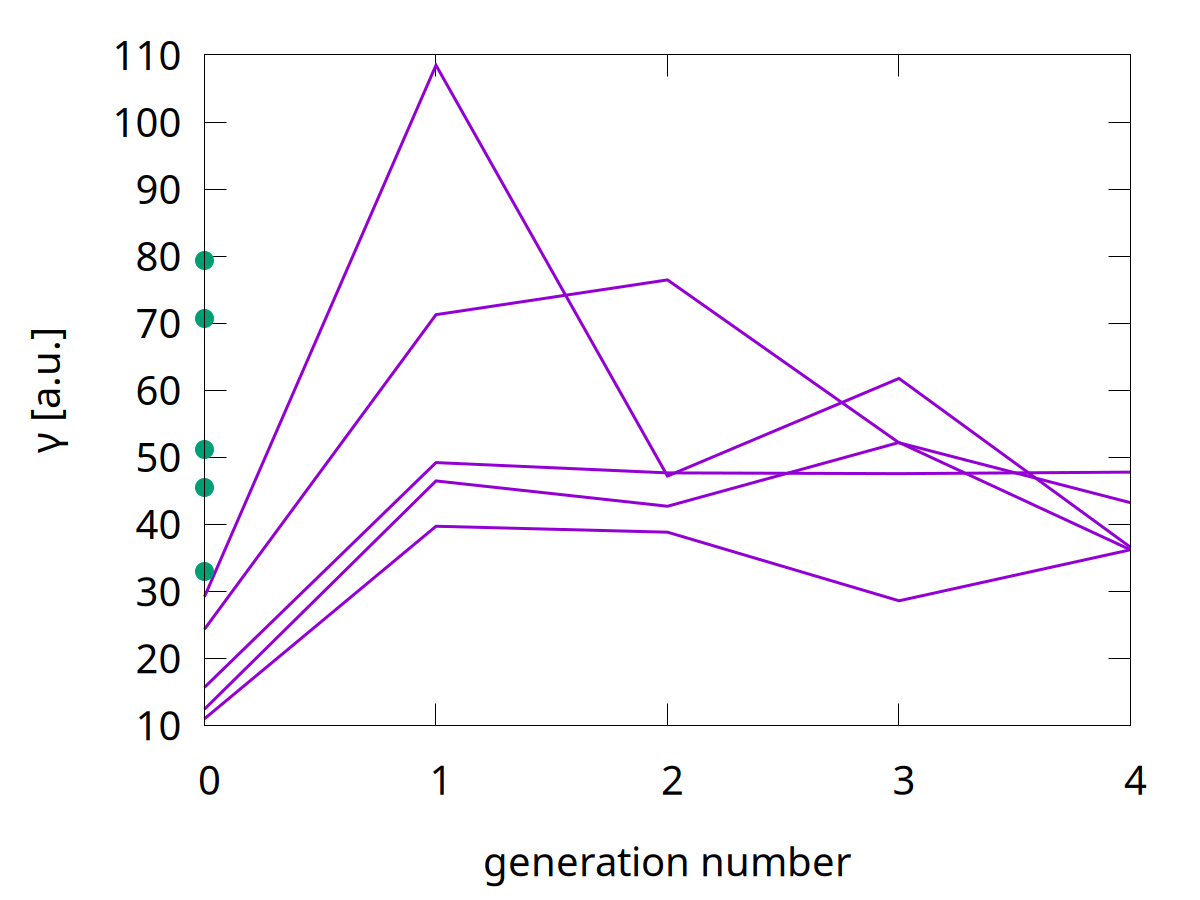
\includegraphics[width=.98\textwidth]{Pics/stats/gen-G.png}
        \caption{} \label{fig:emma-G-gen}
    \end{subfigure}
    \begin{subfigure}{.44\textwidth}
        \centering
        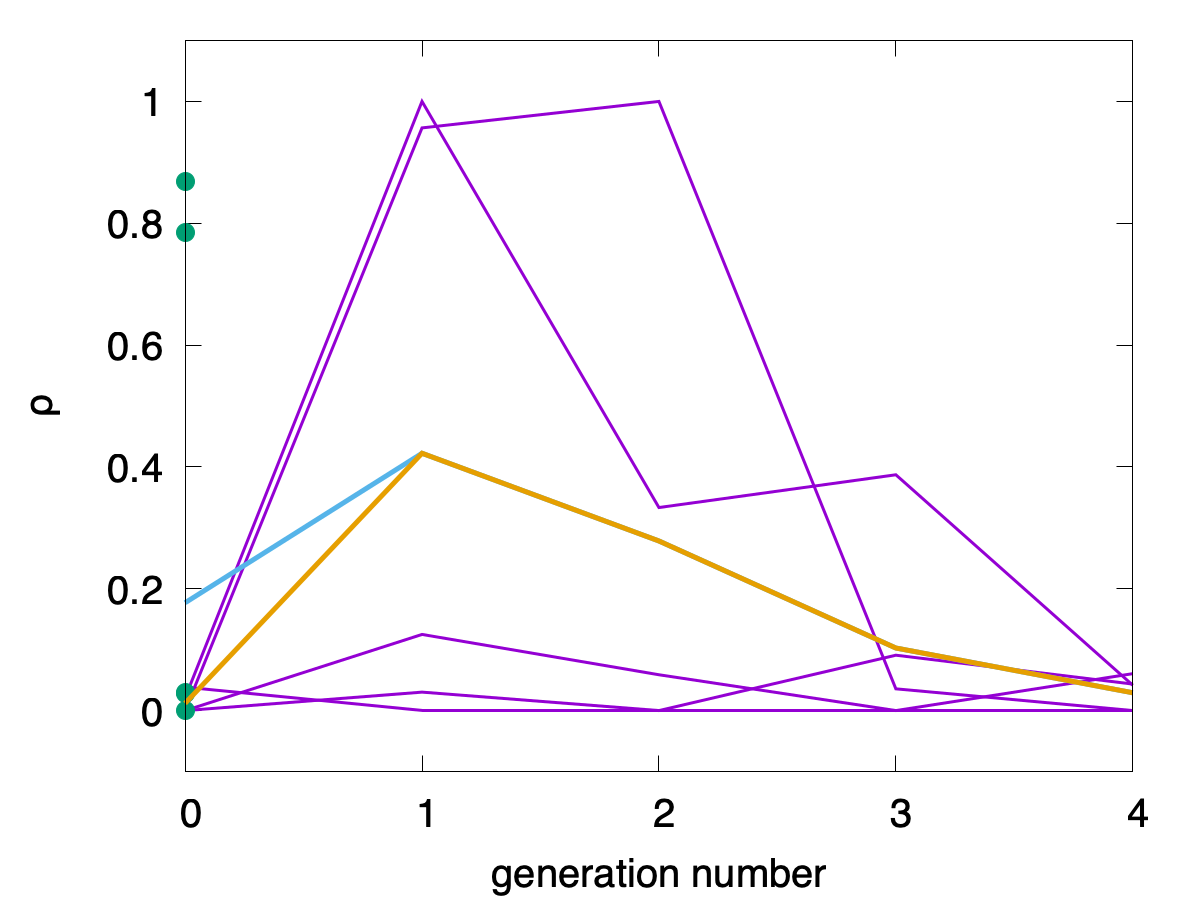
\includegraphics[width=.98\textwidth]{Pics/stats/gen-phd.png}
        \caption{} \label{fig:emma-phd-gen}
    \end{subfigure}
    \begin{subfigure}{.44\textwidth}
        \centering
        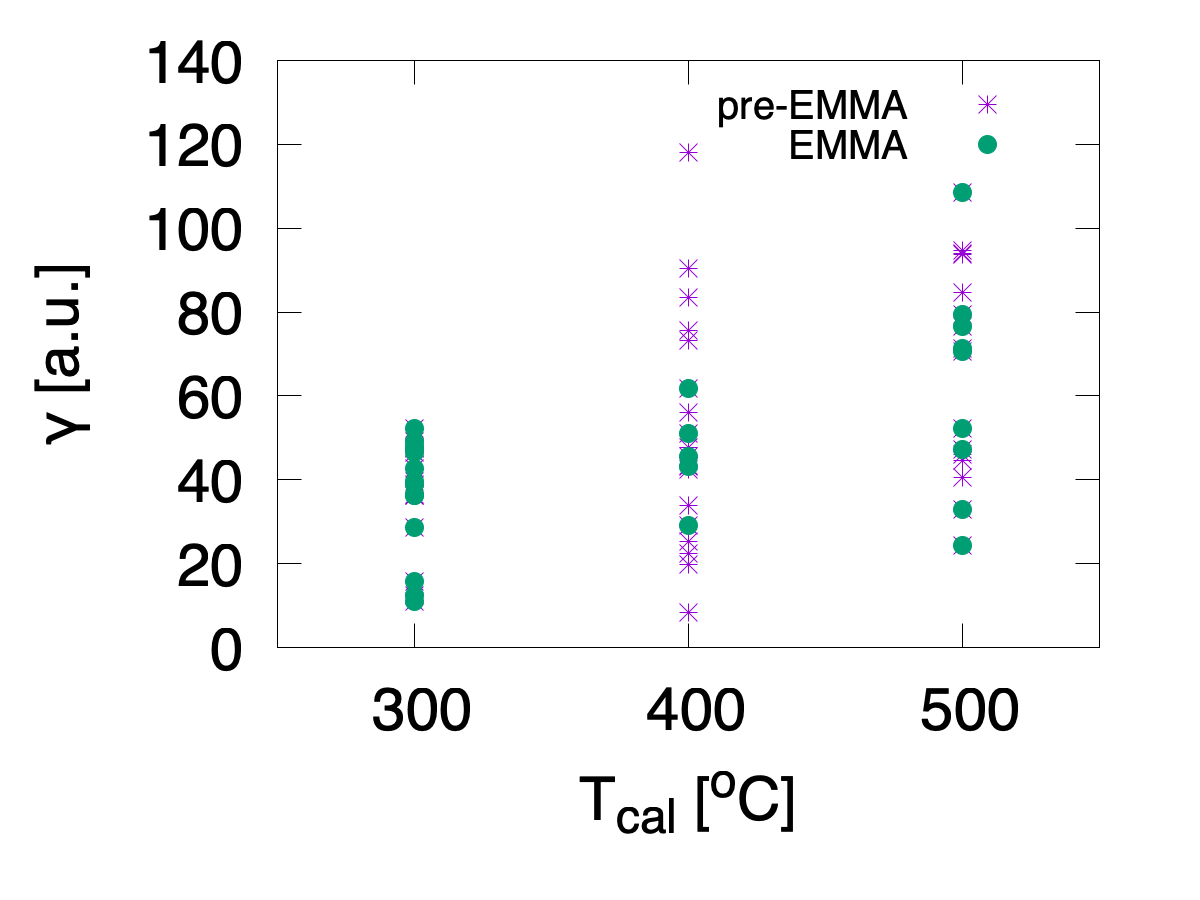
\includegraphics[width=.98\textwidth]{Pics/stats/G-tcal.png}
        \caption{} \label{fig:g-tcal}
    \end{subfigure}
    \begin{subfigure}{.44\textwidth}
        \centering
        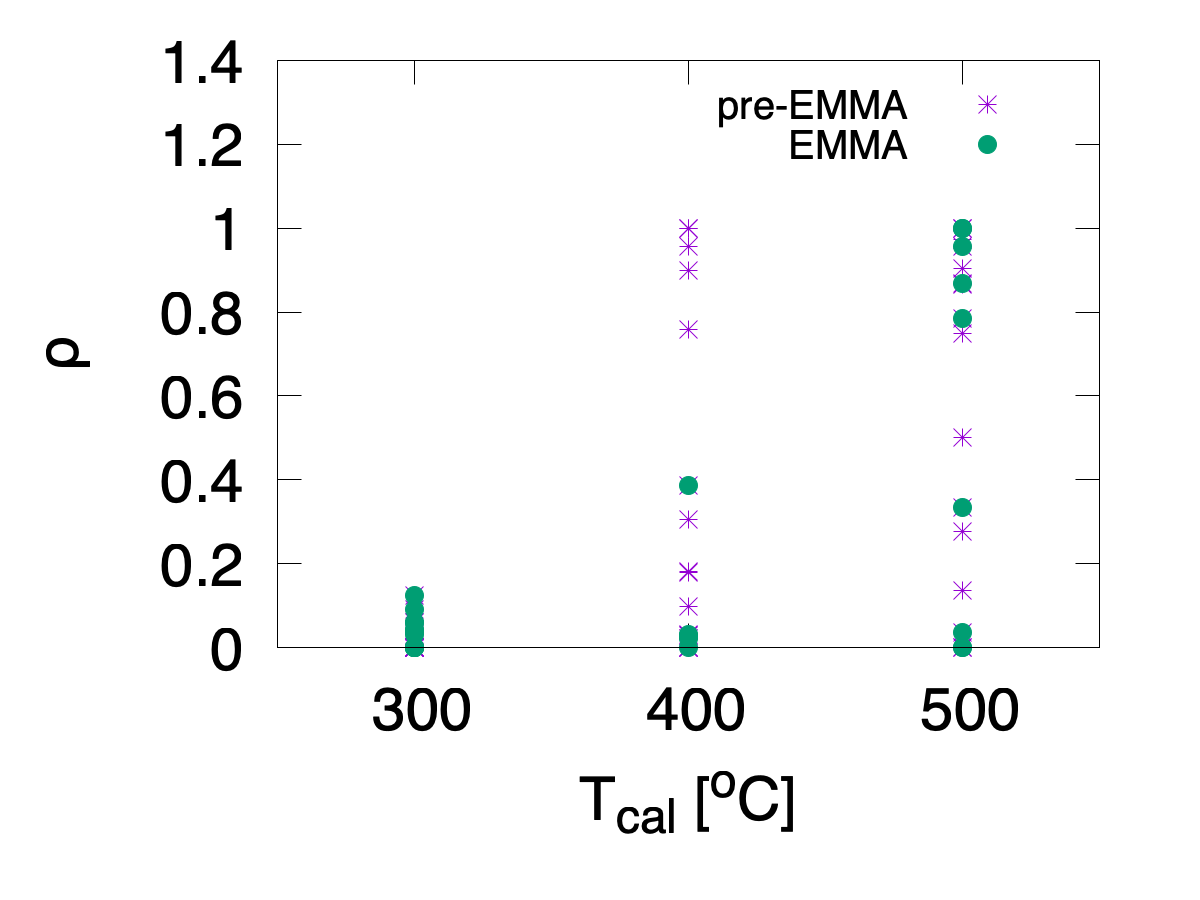
\includegraphics[width=.98\textwidth]{Pics/stats/phd-tcal.png}
        \caption{} \label{fig:phd-tcal}
    \end{subfigure}
	\caption{
		(a)~calculated conductance measures~$\gamma$ of each particle against the generation number %blue shows average for each generation and yellow shows average of each generation without discarded particles from initial generation. 
		(b)~calculated pin hole density~$\rho$ of each particle against the generation number %blue shows average for each generation and yellow shows average of each generation without discarded particles from initial generation. 
		(c)~calculated conductance measures~$\gamma$ against calcination temperature $T_{cal}$
		(d)~calculated pin hole density~$\rho$ against calcination temperature $T_{cal}$
	change colors }

    \label{fig:emma-gen}
\end{figure}

%%% EQUATION 
%\subsection{Equation}
Equations~(\ref{eq:emma-phd3})--(\ref{eq:emma-vcal3}) and (\ref{eq:emma-phd4})--(\ref{eq:emma-vcal4}) represent the regression functions at $t=3$ and $t=4$, respectively, rounded to 2 significant digits.
%$h(x)$ is the hinge function (also called a rectifier function) of the simple form $h(x) = max(0,x)$. 
The expression $h(n_L-6)$ translates into layer count only has an influence if larger than 6 
and $h(6-n_L)$ into layer count influential only if under 6.
%
The first thing to notice is that prediction functions of each generation depend on the same variables. 
%This means that the algorithm must decide on the variables which explain the most variance independent of optimization weights.
This stems from the fact that the algorithm chooses a single minimal set of basis functions to predict all dependent variables. 
%
%\td{Knowing this, makes the decision of adding $n_L$ and $v_{cal}$ as \textit{optimizands} rather unfortunate. %highly questionable. 
%\td{This makes including $n_L$ and $v_{cal}$ as dependent variables unfortunate decisions with hindsight.}
%As the \gls{mars} algorithm is greedy,
%Different independent variables compete to be used as \gls{bf} in the prediction functions because of the greediness of the \gls{mars} algorithm. 
%}

\begin{align}
%
%    \label{eq:emma-phd1}
%    \hat{\rho}_1 &= -0.52 + 2.3\cdot 10^{-5} \cdot  T_{C}\cdot T_{cal} + 0.00080 \cdot h(6-n_L)\cdot T_{cal}\\
%    \label{eq:emma-G1}
%    \hat{\gamma}_1 &= -26  + 0.0025 \cdot T_{C}\cdot T{cal}  +  0.056 \cdot  h(6-n_L)\cdot T_{cal} \\
%    \label{eq:emma-layr1}
%    \hat{n_L}_1 &= 7.1 + 8.1\cdot 10^{-5} \cdot T_{C}\cdot T_{cal} -  0.0056 \cdot  h(6-n_L)\cdot T_{cal}\\
%    \label{eq:emma-vcal1}
%    \hat{v}_{cal,1} &= 19 - 0.00025 \cdot  T_{C}\cdot T_{cal} - 0.0055 \cdot  h(6-n_L)\cdot T_{cal}\\
%
%    \label{eq:emma-phd2}
%    \hat{\rho}_2 &= 0.23\\
%    \label{eq:emma-G2}
%    \hat{\gamma}_2 &= 47\\
%    \label{eq:emma-layr2}
%    \hat{n_L}_2 &= 7.3\\
%    \label{eq:emma-vcal2}
%    \hat{v}_{cal,2} &= 10\\
%
    \label{eq:emma-phd3}
    \hat{\rho}_3 &= 0.075  -   0.0014 \cdot  v_{cal}  +    0.18 \cdot  h(6-n_L)  + 3.9\cdot 10^{-06} \cdot  v_{cal}\cdot T_{cal} \\
    \label{eq:emma-G3}
    \hat{\gamma}_3 &= 43  -   0.097 \cdot  v_{cal}  +     10 \cdot  h(6-n_L)  + 0.00026 \cdot  v_{cal}\cdot T_{cal} \\
    \label{eq:emma-layr3}
    \hat{n_L}_3 &= 9.9  - 0.00064 \cdot  v_{cal}  -     2.7 \cdot  h(6-n_L)  - 1.3\cdot 10^{-06} \cdot  v_{cal}\cdot T_{cal} \\
    \label{eq:emma-vcal3}
    \hat{v}_{cal,3} &= -5.2\cdot 10^{-15}  +   0.016 \cdot  v_{cal}  + 1.3\cdot 10^{-15} \cdot  h(6-n_L)  + 3.9\cdot 10^{-21} \cdot  v_{cal}\cdot T_{cal} \\
%
    \label{eq:emma-phd4}
    \hat{\rho}_4 &=  -0.87 + 0.0047 \cdot  T_{cal} - 0.00036 \cdot  n_L\cdot T_{cal}  +  0.0024 \cdot  h(n_L-6)\cdot T_{C} \\
    \label{eq:emma-G4}
    \hat{\gamma}_4 &=     -19 + 0.28 \cdot  T_{cal}  - 0.022 \cdot  n_L\cdot T_{cal}  +  0.16 \cdot  h(n_L-6)\cdot T_{C} \\
    \label{eq:emma-layr4}
    \hat{n_L}_4 &=  6.8 - 0.014 \cdot  T_{cal}  + 0.0018 \cdot  n_L\cdot T_{cal}  + 0.0060 \cdot  h(n_L-6)\cdot T_{C} \\
    \label{eq:emma-vcal4}
    \hat{v}_{cal,4} &=  29 - 0.052 \cdot  T_{cal}  + 0.0011 \cdot  n_L\cdot T_{cal}  -  0.011 \cdot  h(n_L-6)\cdot T_{C} 
\end{align}

The coefficients in equations (\ref{eq:emma-phd3}) and (\ref{eq:emma-G3}) have the same signs and differ by a factor of roughly 100.
This difference in magnitude fits the data well since the maxima of $\rho$ and $\gamma$ are separated by rough factor of 100 (see figure~\ref{fig:emma-gen} and appendix~\ref{sec:app-emma}). %, but the positive influence of the layer count $n_L$ is counter intuitive 
%as one would expect more layers to be more insulating and thus result in lower conductance and a lower probability of holes going all the way trough the \gls{zro} layers. %pin hole density. 
The coefficients of the $v_{cal} \cdot T_{cal}$ interaction in equations (\ref{eq:emma-phd3}) and (\ref{eq:emma-G3}) 
seem low, but the interaction has -- considering the minimum value of the interaction of $300 \cdot 120 =$  \num{36000} -- several orders of magnitude higher influence on $\rho_3$ and $\gamma_3$ than the $h(6-n_L)$ term. 
%It's positive the hinge
It is astonishing that the knot of the hinge function for equations (\ref{eq:emma-phd3})--(\ref{eq:emma-vcal3}) was chosen so low; 
basically only including the influence of the lowest layer count $n_L=4$.
Meaning for equations (\ref{eq:emma-phd3}) and (\ref{eq:emma-G3}), that the lowest layer count produces worse samples which is intuitive, but more than 6 layers do not improve the insulation. 
Encouragingly, the calcination heating rate $v_{cal}$ (see equation (\ref{eq:emma-vcal3})) has been predicted perfectly within numerical precision. 

%%% T=4
The coefficients of equations (\ref{eq:emma-phd4}) and (\ref{eq:emma-G4}) show the same pattern 
as equations (\ref{eq:emma-phd3}) and (\ref{eq:emma-G3}): identical signs and factor 100. 
%The choice of basis functions in combination with their coefficient signs seems more plausible
%for (\ref{eq:emma-phd4}) and (\ref{eq:emma-G4}) than for (\ref{eq:emma-phd3}) and (\ref{eq:emma-G3}). 
%$n_L$ decreases $\hat{\gamma}$ and $\hat{\rho}$ and additionally, the lowest $n_L$ increases the two \textit{optimizands}. 
%
% TCAL ON OPTIMIZANDS
The influence of $T_{cal}$ on the measures of conductance ($\hat\rho$ and $\hat\gamma$) is highly interesting. 
It was expected that 
calcination temperatures under \oc{400} do not suffice to produce compact layers (corresponding to $+h(400-T_{cal})$)
and 
that therefore the resulting layer does not insulate well if $T_{cal}$ is low (under \oc{400}). 
The opposite is the case, though. % (see figures \ref{fig:g-tcal} and \ref{fig:phd-tcal}).
%This would correspond to $+h(400-T_{cal})$
%The \td{original recipe by Hu et al.\cite{Hu2016} used \oc{500} (but to produce Al2O3, so not a surprise? or?)} and thus even \oc{400} are low.
\textit{Optimizands} $\hat\rho$ and $\hat{\gamma}$ increase with higher calcination temperature 
according to equations~(\ref{eq:emma-phd4}) and (\ref{eq:emma-G4}) (see also figures~\ref{fig:g-tcal} and \ref{fig:phd-tcal}), 
ergo the resistance decreases and the conductance increases with increasing calcination temperature contrary to expectations.

%
% DESCRIBE COEFFICIENTS
Furthermore, the coefficient of the $T_{cal}$ term is the largest of all terms on $\hat{\rho}$ (\ref{eq:emma-phd4}) and $\hat{\gamma}$ (\ref{eq:emma-G4}); interestingly also on $\hat{n_L}$ (\ref{eq:emma-layr4}) and $\hat{v}_{cal}$ (\ref{eq:emma-vcal4}).
The coefficient of the $n_L\cdot T_{cal}$ interaction is about a tenth in size of the $T_{cal}$ coefficient, 
but has the extra factor $n_L$ (range: 4--12), resulting in the products of coefficients and process variables being in the same order of magnitude for $T_{cal}$ and $T_{cal}\cdot v_{cal}$ terms.
It can be noted that the coefficient of the $n_L\cdot T_{cal}$ interaction always has contrary sign to $T_{cal}$ coefficient in equations~(\ref{eq:emma-phd4})--(\ref{eq:emma-vcal4}). 
This negative correlation could hint a compenzation of the overestimated influence of $T_{cal}$ on the \textit{optimizands}.
Similarly, signs of coefficients of $n_L \cdot T_{cal}$ and $h(n_L -6) \cdot T_{C}$ correlate negatively in equations~(\ref{eq:emma-phd4})--(\ref{eq:emma-vcal4}) and the product of coefficients and input variables are again similar in order of magnitude. 
%It should be doubted, though, that the $layr$ only appears as interaction term 
%together with $T_{cal}$ and $T_{C}$, which seems rather than an artefact. 
%
%It seems rather an artefact of noise that the $n_L$ only appears as interaction 
%with $T_{cal}$ and $T_{C}$. 
%From the analysis of coefficients it can be said, that the most important factor according to EMMA is $T_{cal}$, followed by $n_L$, then $T_{C}$ and then the rest of the independent variables. 
The process variables $T_{cal}$ and $n_L$ appear as \gls{bf}s in generation 3 and 4, whereas $v_{cal}$ only appears in generation 3's \gls{rf}s and $T_{C}$ only in generation 4's \gls{rf}s.
This can hint the importance of these variables in the process. 
%I highly doubt though that the specific interactions proposed by EMMA are indeed meaningful. 

%%% MSE
For each generation the \gls{mse} was calculated for which only samples 
from the optimization were used which were available at the time of prediction. 
That means 15, 20, 25 and 30 samples 
%for $t=0$, 15 samples for $t=1$ and 30 samples for $t=4$ 
were used to calculate \gls{mse}s at $t=1,2,3,4$, respectively (compare with table~\ref{tab:emma-Gb}).
The \gls{mse}s are 64, 158, 54 and 50 for $t=1,2,3,4$, respectively. 
It is interesting that although prediction functions for $t=3$ predicted $v_{cal}$ perfectly, the combined \gls{mse} for $t=4$ is lower. 
The high \gls{mse} at $t=2$ can be explained by the prediction functions being only constant values. 
Apart from the second generation the \gls{mse} decreases  over time, 
which indicates that the algorithm works. 
This decrease in \gls{mse} might be attributed to overfitting, though, since prediction and validation were performed on the same data. 
%The \gls{mse} for each generation was also calculated between predicted values for pre-optimization samples to check for overfitting, 
The \gls{mse} for each generation's prediction function was also calculated for pre-optimization (out-of-sample) samples, which are unseen data. 
The error sank again with each generation (except for the second generation): 102, 118, 58, 50, respectively for $t=1,2,3,4$. 
%This shows 
The decrease of \gls{mse} with out-of-sample data shows that the regularization method 
of the \gls{mars} algorithm in principle works on investigated samples and that decrease of \gls{mse} is not due to overfitting. 
%
%\td{It should be noted, that the validation \gls{mse} for $t=1$ is much higher.}
When comparing the out-of-sample and in-sample \gls{mse}s it can be noted that at $t=1$ the out-of-sample \gls{mse} is close to 1.5 fold of in-sample and at $t=2$ vice versa.
%The high validation \gls{mse} for $t=1$ (nearly 1.5 fold instead of circa 1 fold of \gls{mse}) 
This shows the poor prediction ability at the beginning of the optimization which improved with generations.
This decrease in validation (out-of-sample) \gls{mse} supports the hypothesis stated at the beginning of this section: 
the measure of conductance was underestimated and the estimate improved over time (see table~\ref{tab:emma-pred-G}).
%\td{why is \gls{mse} higher with higher values? No homoscedasticity ( equality of variance)?
%Or rather \gls{mse} at $t=2$ high because \gls{rf}s at $t=2$ poor and gen=2 samples are chosen with help of \gls{rf} at $t=2$? 
%}

%%% PROBLEMS 
Even though the main \textit{optimizands} were minimized as required, the \gls{rf}s were not satisfactory. 
The two main problems were too many independent variables and too many dependent variables. 
Both seem closely related and overcomplicate the optimization, but both come with their own implications. 
Too many independent variables make it harder to distinguish variance due to random error (e.g. unmeasured and uncontrolled variables) from variance due to dependency. % of chosen dependent variables. 
The difficulty of identifying meaningful correlation is mainly owed to the curse of dimensionality\cite{friedman1988fitting} which makes it hard to collect enough data for each dimension. 
%
%In the here presented optimization model 
%the data points per independent variable 
%(events per predictor variable EPV) are as low as 5. 
The \gls{epv} (data points per independent variable) are as low as 5 in the here presented optimization. % model and data acquisition method
By eliminating three independent variables the \gls{epv} could rise to 10, which is stated 
as rule of thumb for multivariate regression\cite{vittinghoff2007relaxing}. 
The results obtained with limited sample number deliver remarkable insight %are quite respectable 
comparing to an \gls{epv} of 20-50 stated in the original \gls{mars} paper\cite{friedman1991multivariate} 
and an \gls{epv} of around 20 in the original \gls{emma} paper\cite{villanova2010function}. 
%In the original \gls{emma} paper\cite{villanova2010function} the \gls{epv} is 20.
%\td{In the original \gls{mars} paper\cite{friedman1991multivariate} the model is said 
%to work well on 20-50 events per predictor varibale.
%In the current model EPV are around 5, which is even low for a conservative 
%rule of thumbs of 10-15 EPV\cite{vittinghoff2007relaxing}.
%Not even rule of thumb of 10 EPV \cite{vittinghoff2007relaxing}
%Inspect \cite{friedman1988fitting,friedman1991multivariate} for further \gls{mars} discussion. 
%"The curse-of-dimensionality is fundamental and cannot be directly overcome."- Friedman 1988\cite{friedman1988fitting}.
%}
%

%On the other side, 
The main problem about too many dependent variables specific to this optimization procedure 
is that the same set of basis functions will be used to predict \textbf{all} \textit{optimizands}.
This leads to competition between the \gls{bf}s, as not all dependent variables may depend on the same independent variables. 
This effect is reinforced by the choice of two independent variables as dependent variables. % (IVDV). 
Independent variables as dependent variables will likely be chosen in \gls{bf}s, 
for including them in the \gls{rf}s is an easy way to reduce the \gls{mse} and improve prediction accuracy.
\enlargethispage{\baselineskip}
These \gls{bf}s then "take away places" of \gls{bf}s predicting other dependent variables in the \gls{rf}. %\td{(cf. musical chairs)} 
This in turn can lead to wrong predictions and therefore inefficient choice of future samples. 

The two independent variables $v_{cal}$ and $n_L$ were included as \textit{optimizands} for two reasons: 
Maximizing the calcination velocity and minimizing the number of layer application iterations leads to minimization of process time.
The process time optimization would be better placed in a follow up study. 
The second reason for including independent variables as \textit{optimizands} was to check if the model works. 
This idea has two flaws: there is only one set of \gls{bf}s for all \textit{optimizands} and thus 
additional dependent variables not only complicate the model but make it more difficult to predict the actual dependent variables and chose future data points. 
Moreover, $v_{cal}$ and $n_L$ were only considered with 5\% weight in the overall objective function.
The second flaw is that there are obviously better methods to assess the quality of a model than to make it more complex. 
%Good alternatives would have been leave-one-out or cross validation.
Validation methods for sparse data include re-sampling via leave-one-out or $k$-fold cross validation\cite{kartam1997artificial}.



\iffalse
\td{
%%%%%%%%%%%%%%%%%%%%%%%%%%%%%%%%%%%%%%%%%%%%%%%%%%%%%%%%%%%%%%%%%%%%%%%%%%%%%%%%%%%%%%%%5
%\subsection{how did evolve over time?}
%%%%%%%%%%%%%%%%%%%%%%%%%%%%%%%%%%%%%%%%%%%%%%%%%%%%%%%%%%%%%%%%%%%%%%%%%%%%%%%%%%%%%%%%
\subsection{rational behind including $v_{cal}$ and $n_L$ as optimizands}
}
%
%Three major flaws behind this consideration became obvious with time: 
%
\
\td{
(1) The true function for predicting $v_{cal}$ and $n_L$ are $v_cal*60$ (\oc{}/\h{} instead of \oc{}/\minutes{}) and $n_L$, respectively. 
The algorithm will tend to include those values into the prediction function for 
all dependent variables and possibly exclude others which have more influence 
on $\gamma$ and $\rho$ (see equations (\ref{eq:emma-G4})? And (\ref{eq:emma-phd4})?).
%
(2) The algorithm would be influenced by those values to choose samples, which potentially optimize $v_{cal}$ and/or $n_L$ but not $G$ or $\rho$. 
%
(3) needlessly making the problem more complicate %, important time (around 10\% of the samples) could have been replaced with more insightful samples. 
\begin{itemize}
    \item Every output var is independent of each other, so $v_{cal}$ can act as test 
heating rate was one of the dependent variables with the intention of minimizing the variable. 
It can also be used as test to see how well the EMMA performs (or rather, more precisely MARS).
Even if it didn't influence the fit for the other splines, but it influences the choice of samples therefore it might have slowed down the process
Overall there were too many variables involved for such a small dataset
        that means that adding dependent variables influences \td{previous variables}
\end{itemize}
}

Inspect \cite{friedman1988fitting,friedman1991multivariate} for further \gls{mars} discussion. 
%"The curse-of-dimensionality is fundamental and cannot be directly overcome."- Friedman 1988\cite{friedman1988fitting}.
%}
\fi
